%This is paper.tex

%Write the contents of your paper here.

\newcommand{\degree}{$^\circ$}

\section{Introduction}
Tree volume measurement is one of the many parameters in documenting and profili
ng trees and is at the center of forest inventory. 
% Estimates of tree volume are important for planning timber harvests and modelling carbon sequestration

%I'd delete this part
The use of this information i
s important to companies who need to make smart, profitable decisions but also n
eed to be certain that the choices they make now are maintable in the future. Ho
wever this information also benefits climate modellers, environmental groups and
 governments who want to be able to sustain ecosystems and plan restorations. 
 
 %Unfortunately, estimating tree volume is currently a complex, time-consuming, and expensive procedure.
 To
 be able to accomplish this in forestry, it is a necessity to be able to collect
 large amounts of data easily and on a regular basis. Most methods used today to
 measure individual trees are often done manually with a variety of tools. The u
se of these analogue approaches is expensive, time consuming and in most cases t
he data collected doesn't meet today's standards \cite{digital imaged based tree
 measurement for forest inventory}. 
 
The measurements required for forest inventory can be achieved through a number 
of methods. %the most common method uses what is called a biltmore stick...
One of them is using a so called biltmore stick. A biltmore stick is
 similar to a normal ruler but has been specially modified for measuring trees. 
When standing at a certain distance the user can discern the height of the tree 
by holding the biltmore stick up to their eye and reading the corresponding numb
er. The biltmore stick can also easily be used to measure the DBH of the tree. %define DBH

%i'd eliminate this section
Other ways of measuring tree volume include using a combination of lasers and inc
linometers or by having a person manually climb up the tree and drop a tape meas
ure down to measure the height. 


Despite these relatively simple ways of measurin
g they often leave room for error. That’s why a more common way of getting a pre
cise reading is to cut down trees in the area and then physically measure them
. After the relevant data is collected, one applies a stem-profile taper equation
 that is specific to the species of tree measured. These taper functions are bas %need more explanation about taper functions
ed on numerous measurements and have been refined over the years. The main probl
em with taper functions is that to get an accurate result they need to be callib
rated to the hundreds of local conditions. This again is cost prohibitive and on
ly so much of a forest can be accounted for in the taper function. Even when one
 manages to create a new taper function, it is still far from perfect as all tre
es, even from the same species, differ in shape.

%However, a high-tech startup company named SilviaTerra is trying to change that.
 SilviaTerra, however, is a company willing t
o change that and have already developed several tools for scanning, analyzing a
nd mapping areas of forestry to give accurate results. This is achieved through 
computer exactitude combined with statistical analysis. Recently a new project w %this part is awkwardly phrased
as started, with this research project developing the mathematical back end, to 
allow users to easily get a correct volume measurement by only using their smart
 phone.

This project aims to solve 
the described problem % -> tree volumes by...
using a combination of photo
s taken of the tree, various sensor data from the phone and mathematical computa
tion. This is supposed to then give a accurate result, cheaply and non-destructi
vely. All within the reaches of a mobile phone. % this last sentence is awkward

\section{Background}

\begin{figure}[!htb]
	\minipage{0.45\textwidth}
		\centering
  		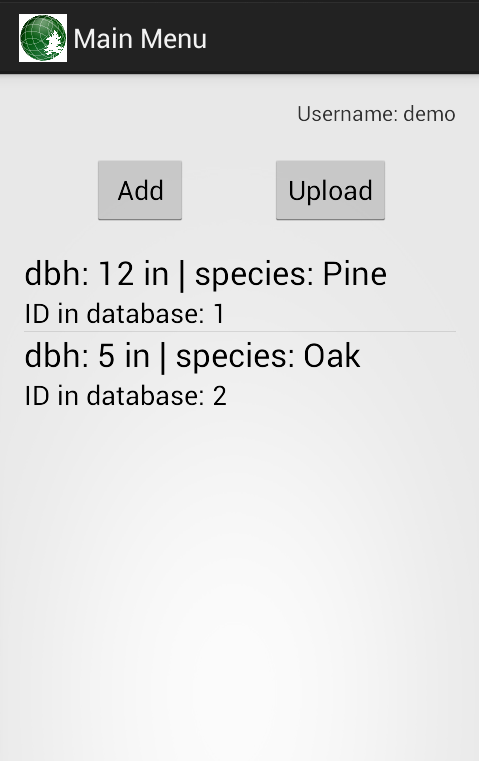
\includegraphics[width=0.65\textwidth]{main.png}
	  	\caption{Homescreen}
  		\label{main}
	\endminipage\hfill
	\minipage{0.45\textwidth}
		\centering
	  	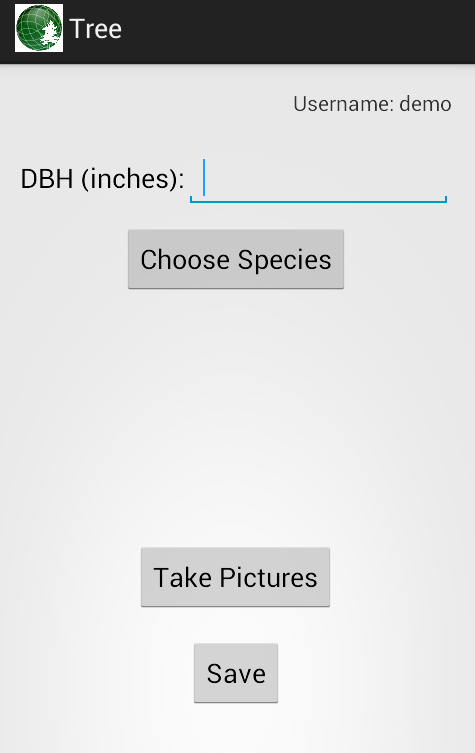
\includegraphics[width=0.65\textwidth]{input.png}
	  	\caption{User input}
  		\label{input}
	\endminipage\hfill
\end{figure}
%not sure you need this part... just stick to describing the bare-minimum needed to understand the measurements
The first thing a person does when accessing the mobile application is to log in
to the system with their user name and password. After that they are prompted wi
th a simple menu where they can either choose to add new trees to their inventor
y or upload them to SilviaTerra's cloud service, figure \ref{main}. 
The data can then later be used with SilviaTerra's other products. 
 
 If the user chooses to ad
d a new tree then they will be asked to enter the tree's DBH and species, \ref{i
nput}. 
\begin{figure}[!htb]
	\minipage{0.45\textwidth}
		\centering
  		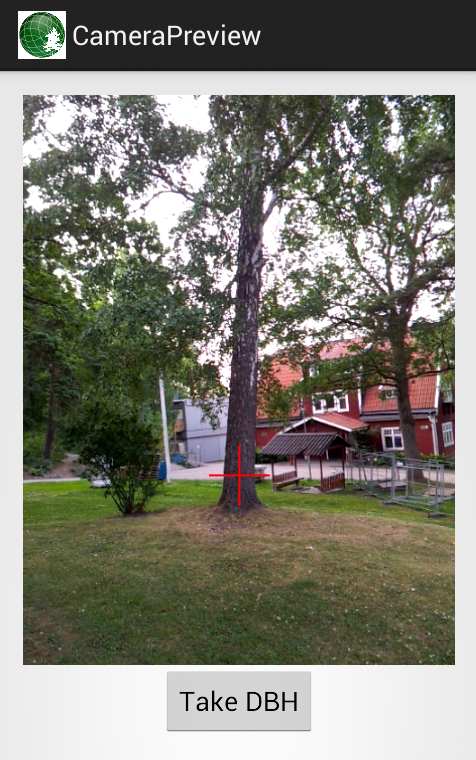
\includegraphics[width=0.75\textwidth]{dbh.png}
	  	\caption{DBH picture}
	  	\label{dbh}
	\endminipage\hfill
	\minipage{0.45\textwidth}
		\centering
	  	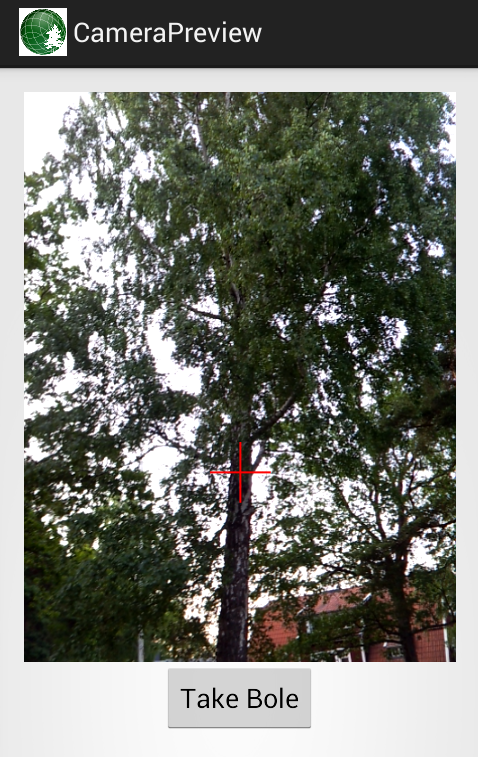
\includegraphics[width=0.75\textwidth]{bole.png}
	  	\caption{Bole picture}
	  	\label{bole}
	\endminipage\hfill
\end{figure}

After that they take two pictures. The interface is quite simple with a cross-ha
ir to show where to point the camera. The first picture is of the actual DBH, fi
gure \ref{dbh}, and the second picture is of the bole of the tree, figure \ref{b
ole}. Between these two pictures the camera will have to be tilted vertically to
 capture the bole. The angle between these two camera positions is recorded thro
ugh the internal gyroscope. %and accelerometers

%explain that, "Now the challenge is to extract useful measurements from these pictures"
% "We need to identify a bunch of points along the trunk of the tree to fit taper equations"
After this stage the user's role in the application 
is done and the pictures are sent to one of SilviaTerra's web servers. Here horiz
ontal lines that run parallel with the bottom of the image are drawn across the 
entire picture. These are drawn at different pixel heights with equal pixel dist
ance in between. 

%Say instead, "to perform this task computationally would be quite difficult and error-prone,
% so instead the company opted to have this task performed manually by workers on Amazon's Mechanical Turk service.
The reason this is done is because computer vision is still an 
experimental technology and is not fully capable yet of being to detect the edge
s of trees with a background of forestry. 

%eliminate this part
Seeing as this is a commercial product
, it would be quite disadvantageous if errors were commonplace. 

%not sure you need this part - maintain focus on the key problem of solving volumes!
So instead the i
mages with the newly drawn lines are then forwarded to Amazon's Mechanical Turk 
service. Just like the name suggests Amazon's Mechanical Turk is meant to be an 
analogy to the 18th century concept of a automated chess board. The service is i
n its simplest form a crowd sourcing internet marketplace where individuals or b
usinesses can request tasks to be completed. Usually the tasks are ones that are
 difficult for computers but easy for humans. 
 
 SilviaTerra creates tasks where pe
ople manually click where the previously drawn lines, cross the edges of the tre
e. Once the points of intersection are identified, their corresponding pixel coo
rdinates are the sent back to the web server. 

%The pixel coordinates that result are then paired with the phone sensor data 
% and input into a program to perform a photogrammetric analysis to derive the taper equations.
The pixel coordinates along with i
nformation from the phone is piped into a program where the volume is then calcu
lated. It is this program that is the main topic of this research paper.

\section{Method}
Once all the required information has been retrieved it is piped into the progra
m that will be calculating the volume. %and taper equations!

The dataset that is used comprises inform
ation about the phone and the results from Mechanical Turk. It is as follows:
\begin{itemize}
	\item DBH length
	\item Horizontal and vertical angle of view
	\item Horizontal and vertical image resolution
	\item Pitch of phone when images are captured
	\item Left and right pixel coordinates from Mechanical Turk
\end{itemize}

\subsection{Distance to tree}
%Try to make this section clearer - it's a bit tedious to understand
The DBH is used as a reference to find all the other measurements. The first unk
nown that must be discovered is the distance to the tree. This distance is paral
lel with the ground. The difference between the x-coordinates of the left and ri
ght pixel that correspond to the DBH is calculated, figure \ref{horizontal_trian
gle}, $X_1$ and $X_2$. Due to the fact that the width of the DBH is now known in
 both pixels and in a physical measurement, the ratio between the two can be det
ermined by dividing the physical distance between $X_1$ and $X_2$ with the numbe
r of pixels betwee them.
\begin{figure}[htp]
\centering
{
	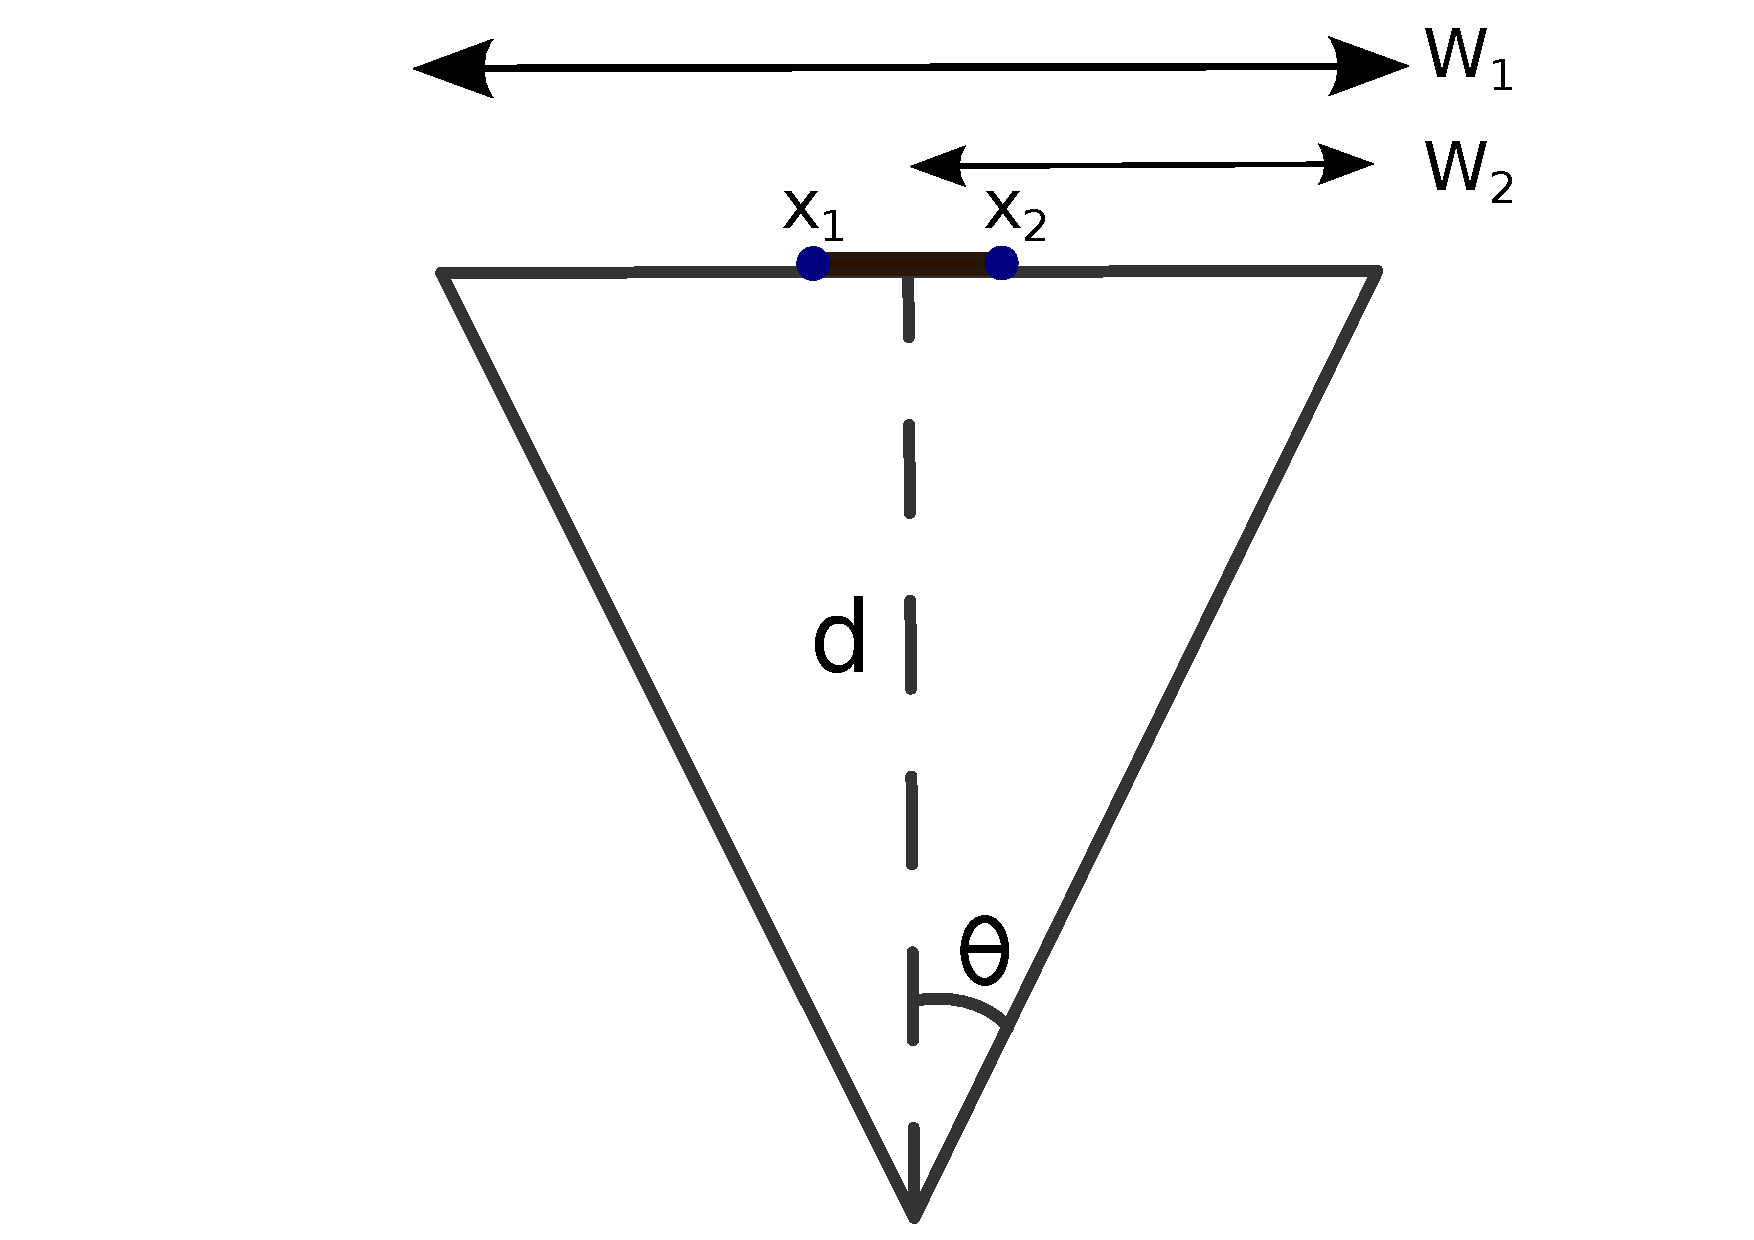
\includegraphics[scale=0.3]{horizontal_triangle.pdf}
	\caption{Birds eye view of horizontal plane}
	\label{horizontal_triangle}
}
\end{figure}
 As seen in figure \ref{horizontal_triangle} an isosceles triangle can be constr
ucted with the horizontal angle of view as the vertex angle. The triangles two c
ongruent legs extend out towards the base of the triangle, $W_1$, which is inlin
e with the tree. To get the length of the base, %(corresponding to <WHAT> in the real world...)
$W_1$, the previously calculated
 scale between pixels and the real world is multiplied with the number of pixels
 in the horizontal resolution of the image. The distance to the tree can easily 
calculated by drawing an extra line that bisects the vertex angle, contriving th %contriving?  how about "resulting in an"
e angle $\theta$ which is exactly half of the angle of view and the actual dista
nce to the tree $d$. This line also divides $W_1$ into $W_2$ and futhermore prod %produces* - parallel tenses
ucing a right angle triangle that can be solved. Finally to actually calculate t
he distance, $d$, $W_2$ is divided by $\tan{\theta}$.


\subsection{Heights and widths} 
\begin{figure}[!htb]
	\minipage{0.45\textwidth}
		\centering
  		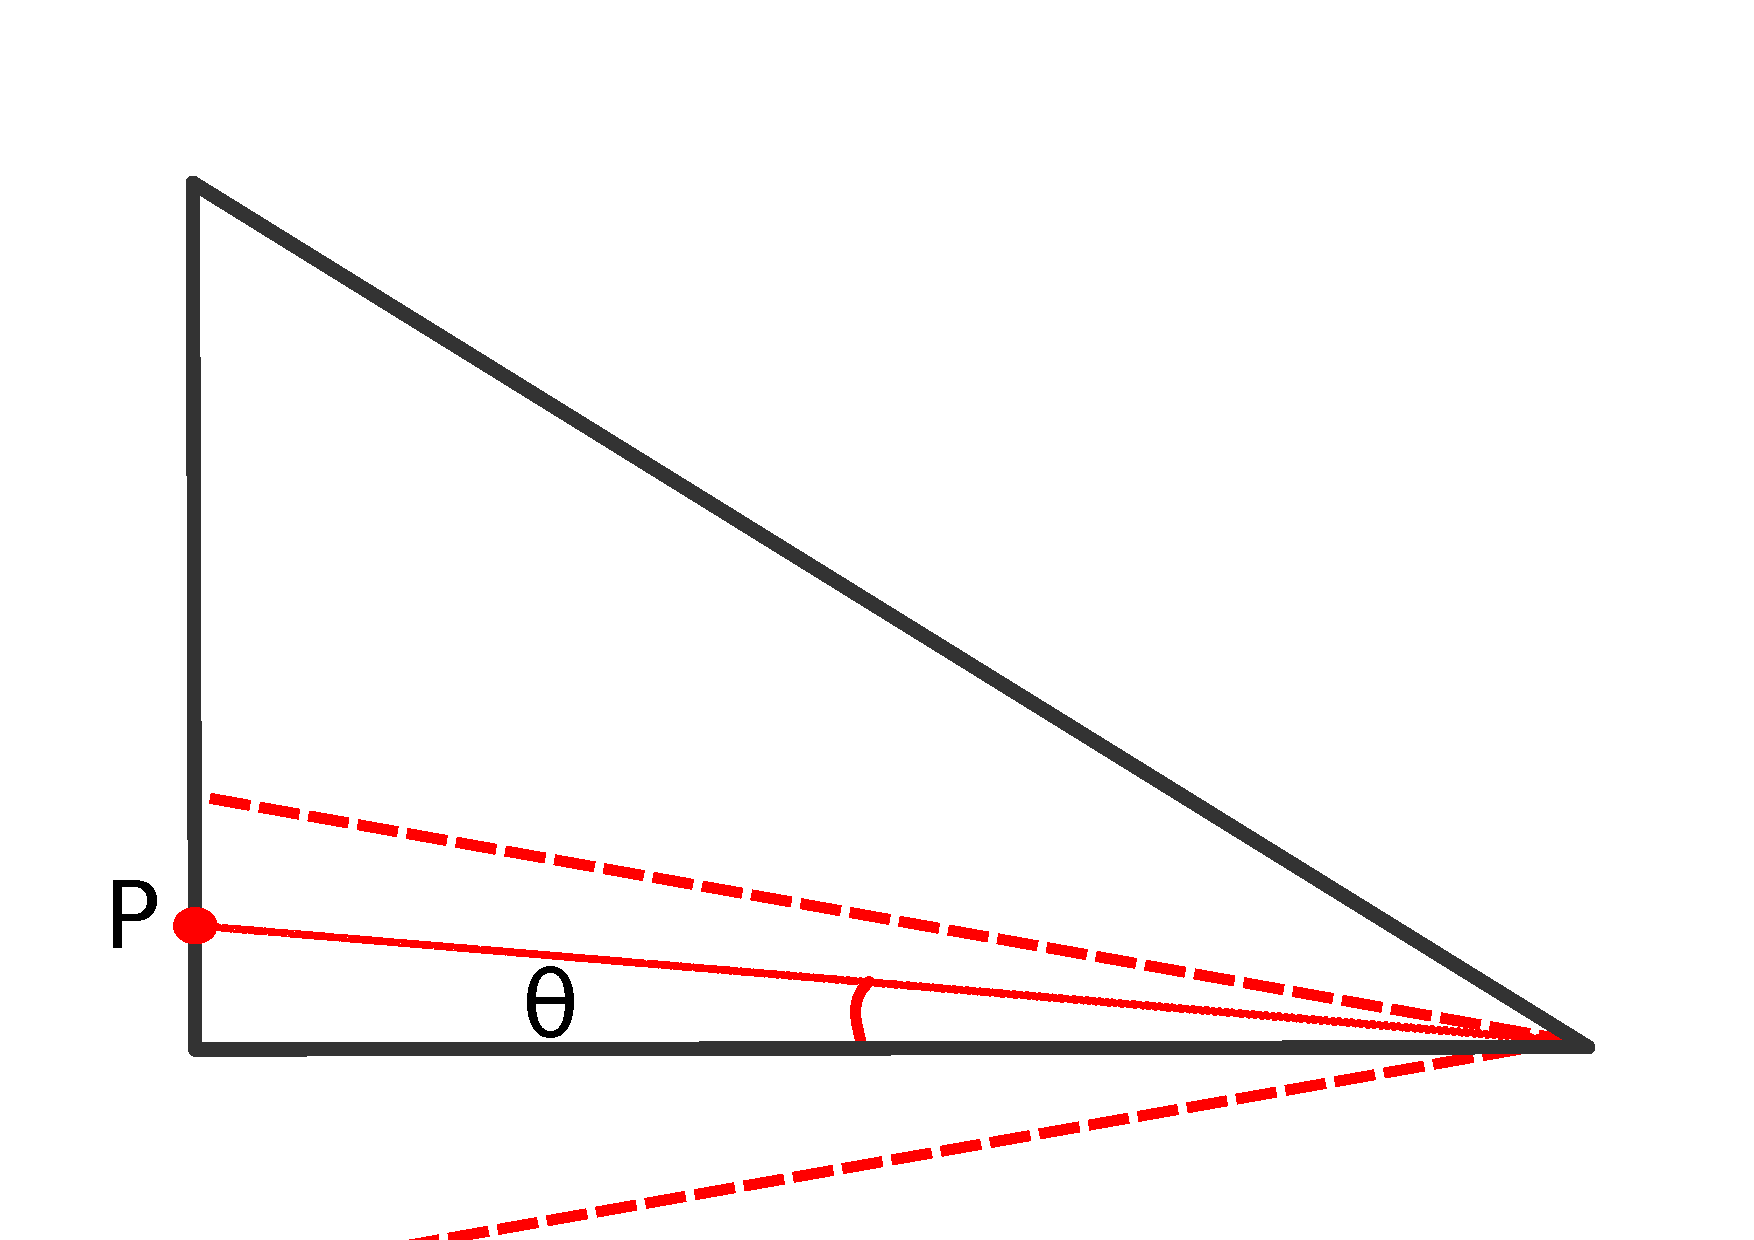
\includegraphics[width=0.9\textwidth]{triangle1.pdf}
	  	\caption{DBH picture}
	  	\label{triangle1}
	\endminipage\hfill
	\minipage{0.45\textwidth}
		\centering
	  	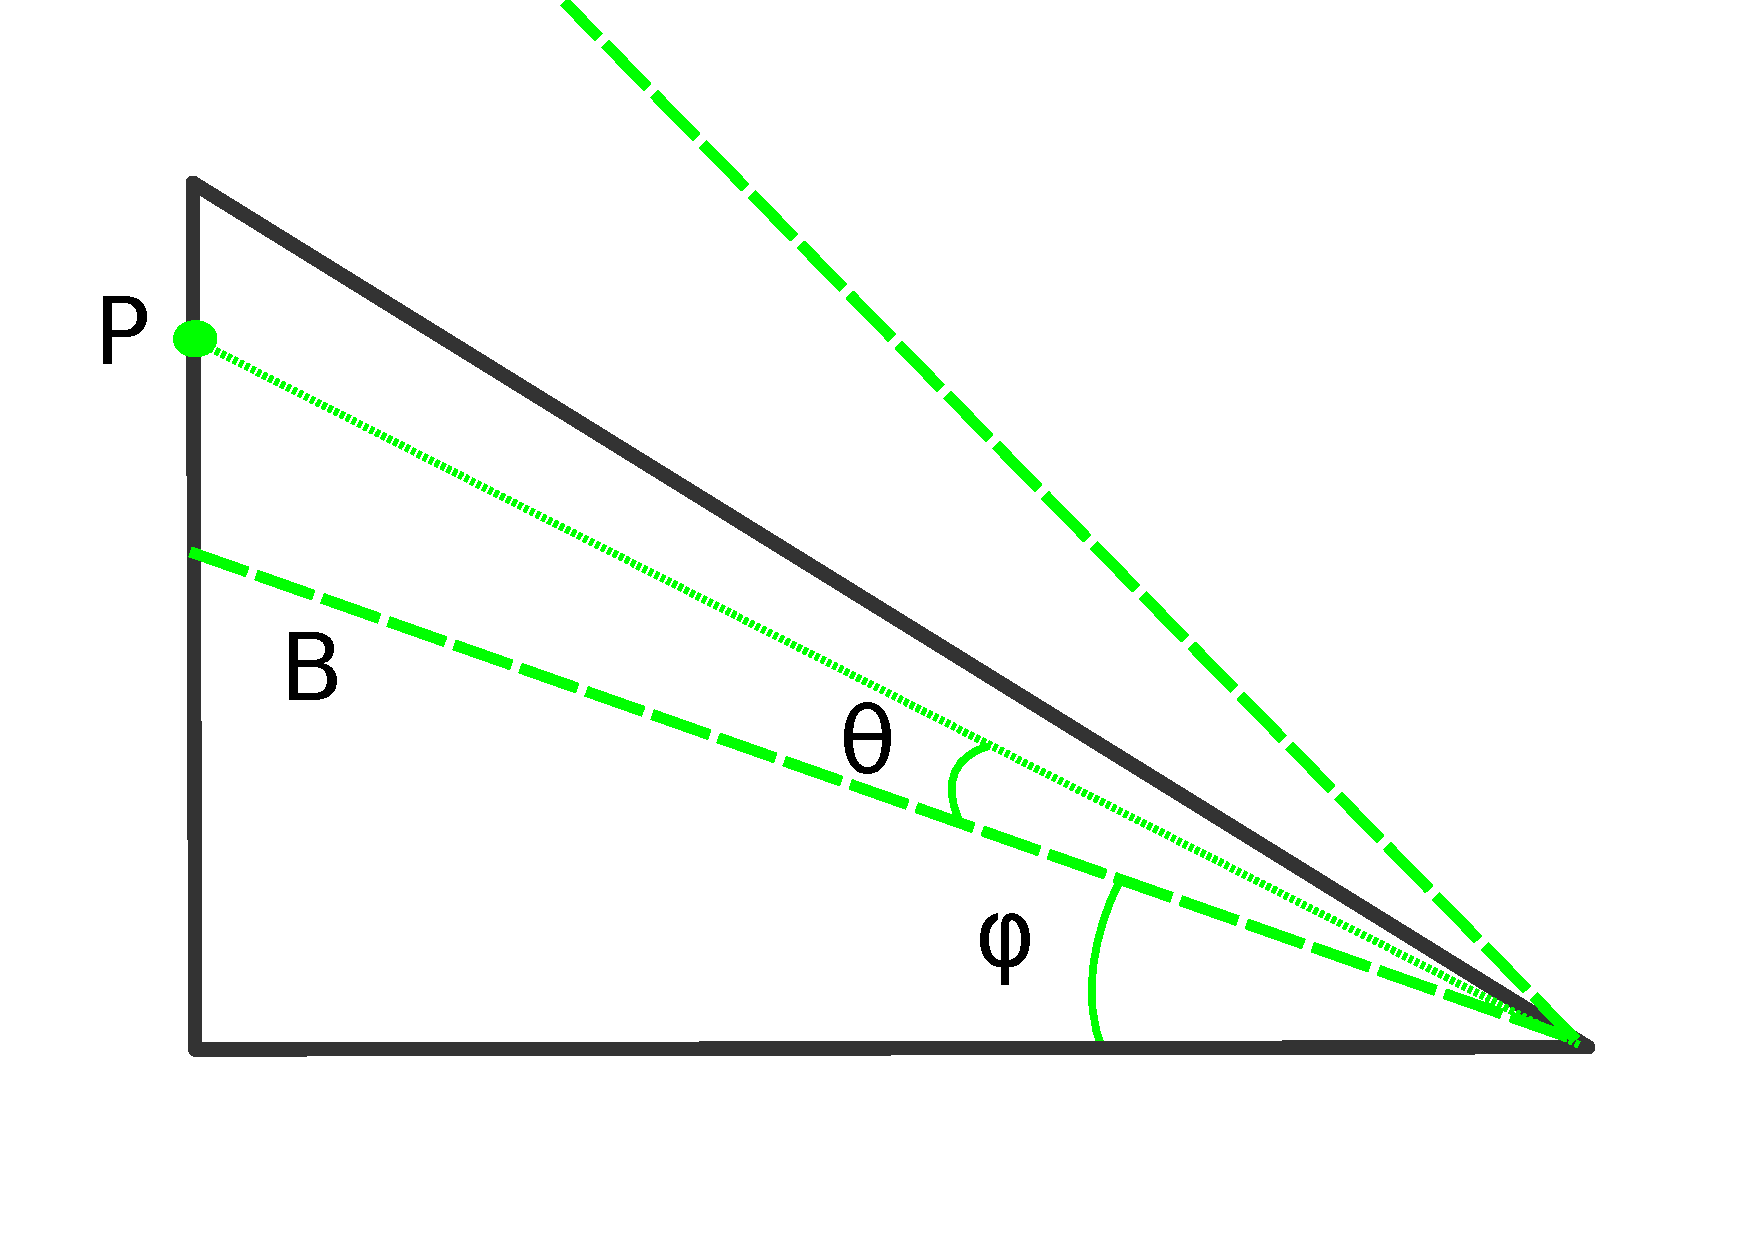
\includegraphics[width=0.9\textwidth]{triangle2.pdf}
	  	\caption{Bole picture}
	  	\label{triangle2}
	\endminipage\hfill
\end{figure}

The next stage is retrieving the real world height to each set pixel coordinates
 as well as the width between them, which will be the diameter of the tree. %at that height
 The 
first step taken is to get the height. The vertical image plate scale, which is %plate scale?  What is an image plate scale?
the ratio between degrees and pixels in the vertical axis, is calculated by divi
ding the vertical resolution of the image with the vertical angle of view. This 
can be done because it is assumed that the silhouette of the tree is on a plane %does this just mean that the tree is straight and doesn't curve towards or away from the image?
in the real world which corresponds to the image plane on the camera sensor. Wit
h this method it is possible to find out the angle to each pixel coordinate, exa
mple $P$ in figure \ref{triangle1} and \ref{triangle2}, in the angle of view. Th
is is angle is denoted by $\theta$ in both figure \ref{triangle1} and \ref{trian
gle2}. However if the pixel coordinate was identified in the bole image, when th
e phone was tilted upwards, then angle between the distance to the tree and the 
lower boundary of the vertical angle of view, $B$, will need to be added, which 
is represented by $\varphi$ in figure \ref{triangle2}. The diagonal distance to 
$P$ is also calculated so that the width can later be determined.

The final part of obataining %spelling!
the parameters for the set of pixel coordinates at 
that height is to calculate the width between them. This is accomplished by empl
oying the method for calculating the distance to the tree, in reverse. In this c
ase what is known in figure \ref{horizontal_triangle} is the distance $d$ and th
e angle $\theta$ but not the width of the tree, $X_1$ to $X_2$. $W_2$ is calcula
ted by multiplying $d$ with $\tan{\varphi}$. $W_2$ is then again multiplied by 2
 and then divided by the number of pixels in the horizontal resolution of the im
age, once more returning the ratio between pixels and the corresponding real wor
ld measurement. To finish off this ratio is the multiplied by the number of pixe
ls between $X_1$ and $X_2$ dispensing %resulting in
the physical width of the tree at that cer
tain height.


\subsection{Volume}
Now the only thing left to produce the final result is to use these newly calcul
ated widths and heights to obtain the total volume. The current implemented meth
od of doing this is by integrating all the points using the trapezoidal rule. Al
l the widths are divided by 2 to get the radius. Then they are squared and multi
plied with $\pi$ to the obtain the basal area at each height. The basal area is 
plotted along with their corresponding heights. The trapezoidal rule then define
s that the area between two points is: $\frac{a_1 + a_2}{2} \times h$. The area 
between all the points is then summed together.


This whole process is looped through for every identified pixel coordinate set u
ntil the width and height is known for all of them. Once that is done, a new loo
p is created for calculating the total volume.

\subsection{Simulation}
To test this method a \emph{virtual tree}, that represented a 4m tall tree,was c
onstructed. This tree was made out of blue tape and tapered off drastically so t
hat the program could be thoroughly tested. Along the tape, points were marked o
ut and the height to them plus the width between corresponding points was measur
ed. Just like in the real application, two pictures were taken. One of the DBH a
nd one of the top of the tree. Each set of points was then identified on the pic
tures and measured in pixels. The parameters were then passed into the program a
nd the results were cross-referenced with the real life measurements.

%do you have a picture?

\newpage

\section{Results}
\begin{table}[h!]
	\begin{center}
		\begin{tabular}{| l c c c c c c r |}		
		\hline
		Measured & 57\degree & 47\degree & 39\degree & 27\degree & 22\degree & 18\degr
ee & 15\degree \\
		\hline
		0 		& 0 	& 0 	& 0 	& 0 	& 0 	& 0 	& 0 	\\
		103 	& 96 	& 100 	& 103 	& 106 	& 113 	& 116 	& 123 	\\
		115 	& 109 	& 113 	& 116 	& 118 	& 125 	& 128 	& 135 	\\
		125 	& 125 	& 129	& 132 	& 134 	& 140 	& 144 	& 150 	\\
		159 	& 142 	& 147 	& 150 	& 151 	& 158 	& 161 	& 167 	\\
		166 	& 158 	& 163 	& 166 	& 167 	& 174 	& 175 	& 183 	\\
		183 	& 173 	& 179 	& 181	& 182 	& 189 	& 192 	& 198 	\\
		\hline
		\end{tabular}
		\caption{Heights over DBH}
		\label{heights}
	\end{center}
\end{table}

\begin{table}[h!]
	\begin{center}
		\begin{tabular}{| l c c c c c c r |}
		\hline
		Measured & 57\degree & 47\degree & 39\degree & 27\degree & 22\degree & 18\degr
ee & 15\degree \\
		\hline
		12       & 11.7      & 12.1      & 12.2      & 12.1      & 12.3      & 12.6   
   & 11.9      \\
		27       & 26.8      & 28.0      & 28.4      & 28.2      & 28.5      & 28.4   
   & 28.1      \\
		37       & 36.4      & 37.5      & 38.0      & 37.7      & 38.2      & 38.1   
   & 37.7      \\
		44       & 42.4      & 43.6      & 44.4      & 44.0      & 44.4      & 44.0   
   & 44.4      \\
		52       & 51.3      & 52.7      & 53.5      & 53.0      & 53.4      & 52.9   
   & 53.2      \\
		61       & 60.9      & 62.2      & 63.1      & 62.1      & 62.8      & 62.5   
   & 61.1      \\
		59       & 59.0      & 59.0      & 59.0      & 59.0      & 59.0      & 59.0   
   & 59.0      \\
		\hline
		\end{tabular}
		\caption{Widths over DBH}
		\label{widths}
    \end{center}
\end{table}

\begin{table}[h!]
	\begin{center}
    	\begin{tabular}{| l c c c c c c r |}
    	\hline
		Measured & 57\degree & 47\degree & 39\degree & 27\degree & 22\degree & 18\degr
ee & 15\degree \\
		412222   & 386642    & 396386    & 418370    & 412084    & 433294    & 445401 
   & 445624    \\
		\hline
		\end{tabular}
		\caption{Total volume over DBH}
		\label{volumes}
    \end{center}
\end{table}

\section{Discussion}
\subsection{Error tolerance}
As seen in table \ref{heights} either when the vertical tilt angle is very wide,
 standing close to the tree, or very narrow, standing far away, leads to error. 
It's not clear what is causing this but there a two possible reasons. The first o
ne is that because of the short focal length of the camera and overall poor qual
ity when compared to a real camera, causes various forms of distortion, especial
ly around the edges of the image. When the person is standing close to the tree 
so the vertical tilt angle is over 45\degree, the points tend to lie exactly the
re, around the edges of the image. The distortion then affects these points caus
ing the pixel measurements to be incorrect. The other problem occurs in the dire
ct opposite situation, when the person is standing far away and the angle is ver
y narrow. Naturally what happens is that the resolution of the camera just isn't
 high enough and the pixel measurements just aren't accurate anymore. However mo
st of this distortion seems to only affect the vertical measurements because whe
n looking at table \ref{widths} it is clearly seen that the readings do not stra
y much at all from their actual values. Despite this the deviation in the height
 readings still alters the volume calculations. Ideally a person should stand so
 that the vertical tilt angle lies between 45\degree and 25\degree which is basi
cally means they should stand somewhere between one tree length to two tree leng
th's from the tree.
\subsection{Limitations}
As pointed out in the previous section the main hindrance attatched to this appl
ication is the actual camera. 
\subsection{Future development}
The main area that could be expanded on is the edge detection. As explained in t
he background, today computer vision is still far from perfect. However that wil
l hopefully change in the near future and things like Mechanical Turk can be dro
pped for a more efficient system that produces little to no error and works auto
nomously.

